\section{Evaluation}
\label{sec:evaluation}

We evaluate Cudele on a 15 node cluster, partitioned into 8 object storage
servers, 3 metadata servers, and 2 monitor servers. The object storage servers
double as clients which is fine because clients are CPU and memory bound while
object storage servers are disk IO bound. All daemons run as a single process
which is the default setting for Ceph and the nodes have 2 dual core 2GHz
processors with 8GB of RAM. There are three daemons per object storage server
(one for each disk formatted with XFS) and they share an SSD for the journal.
The nodes are running Ubuntu 12.04.4, kernel version 3.2.0-63 but all
experiments run in Docker containers; this makes it easier to tear down and
re-initialize ({\it e.g.}, dropping the kernel cache) for the cluster between
experiments.

This paper adheres to The Popper
Convention\footnote{\url{http://falsifiable.us}}~\cite{jimenez_popper_2016}, so
experiments presented here are available in the repository for this
article\footnote{\url{https://github.com/michaelsevilla/cudele-popper/tree/}}.
Experiments can be examined in more detail, or even re-run, by visiting the
\texttt{[source]} link next to each figure. That link points to a Jupyter
notebook that shows the analysis and source code for that graph and its parent
folder contains all the associated artifacts.

\subsection{Microbenchmarks}
%\begin{figure*}[tb]
%\centering
%\includegraphics[width=180mm]{graphs/slowdown.png}
%\caption{Compared to the \texttt{create} phase, saving and persisting
%updates (\texttt{create+save} and \texttt{create+save+persist}) experience only
%a 4.79\(\times\) and 8.66\(\times\) slowdown, in the worst case for 100K files.
%In contrast, maintaining \texttt{global} consistency is 905.70\(\times\)
%slower.  The disadvantage of decoupling the namespace is the merge phase where
%updates are applied to the metadata store (\texttt{create+apply}, resulting in a
%905.70\(\times\) slowdown for 100K files.}\label{fig:global-v-decoupled}
%\end{figure*}

\begin{figure}[tb]
\centering
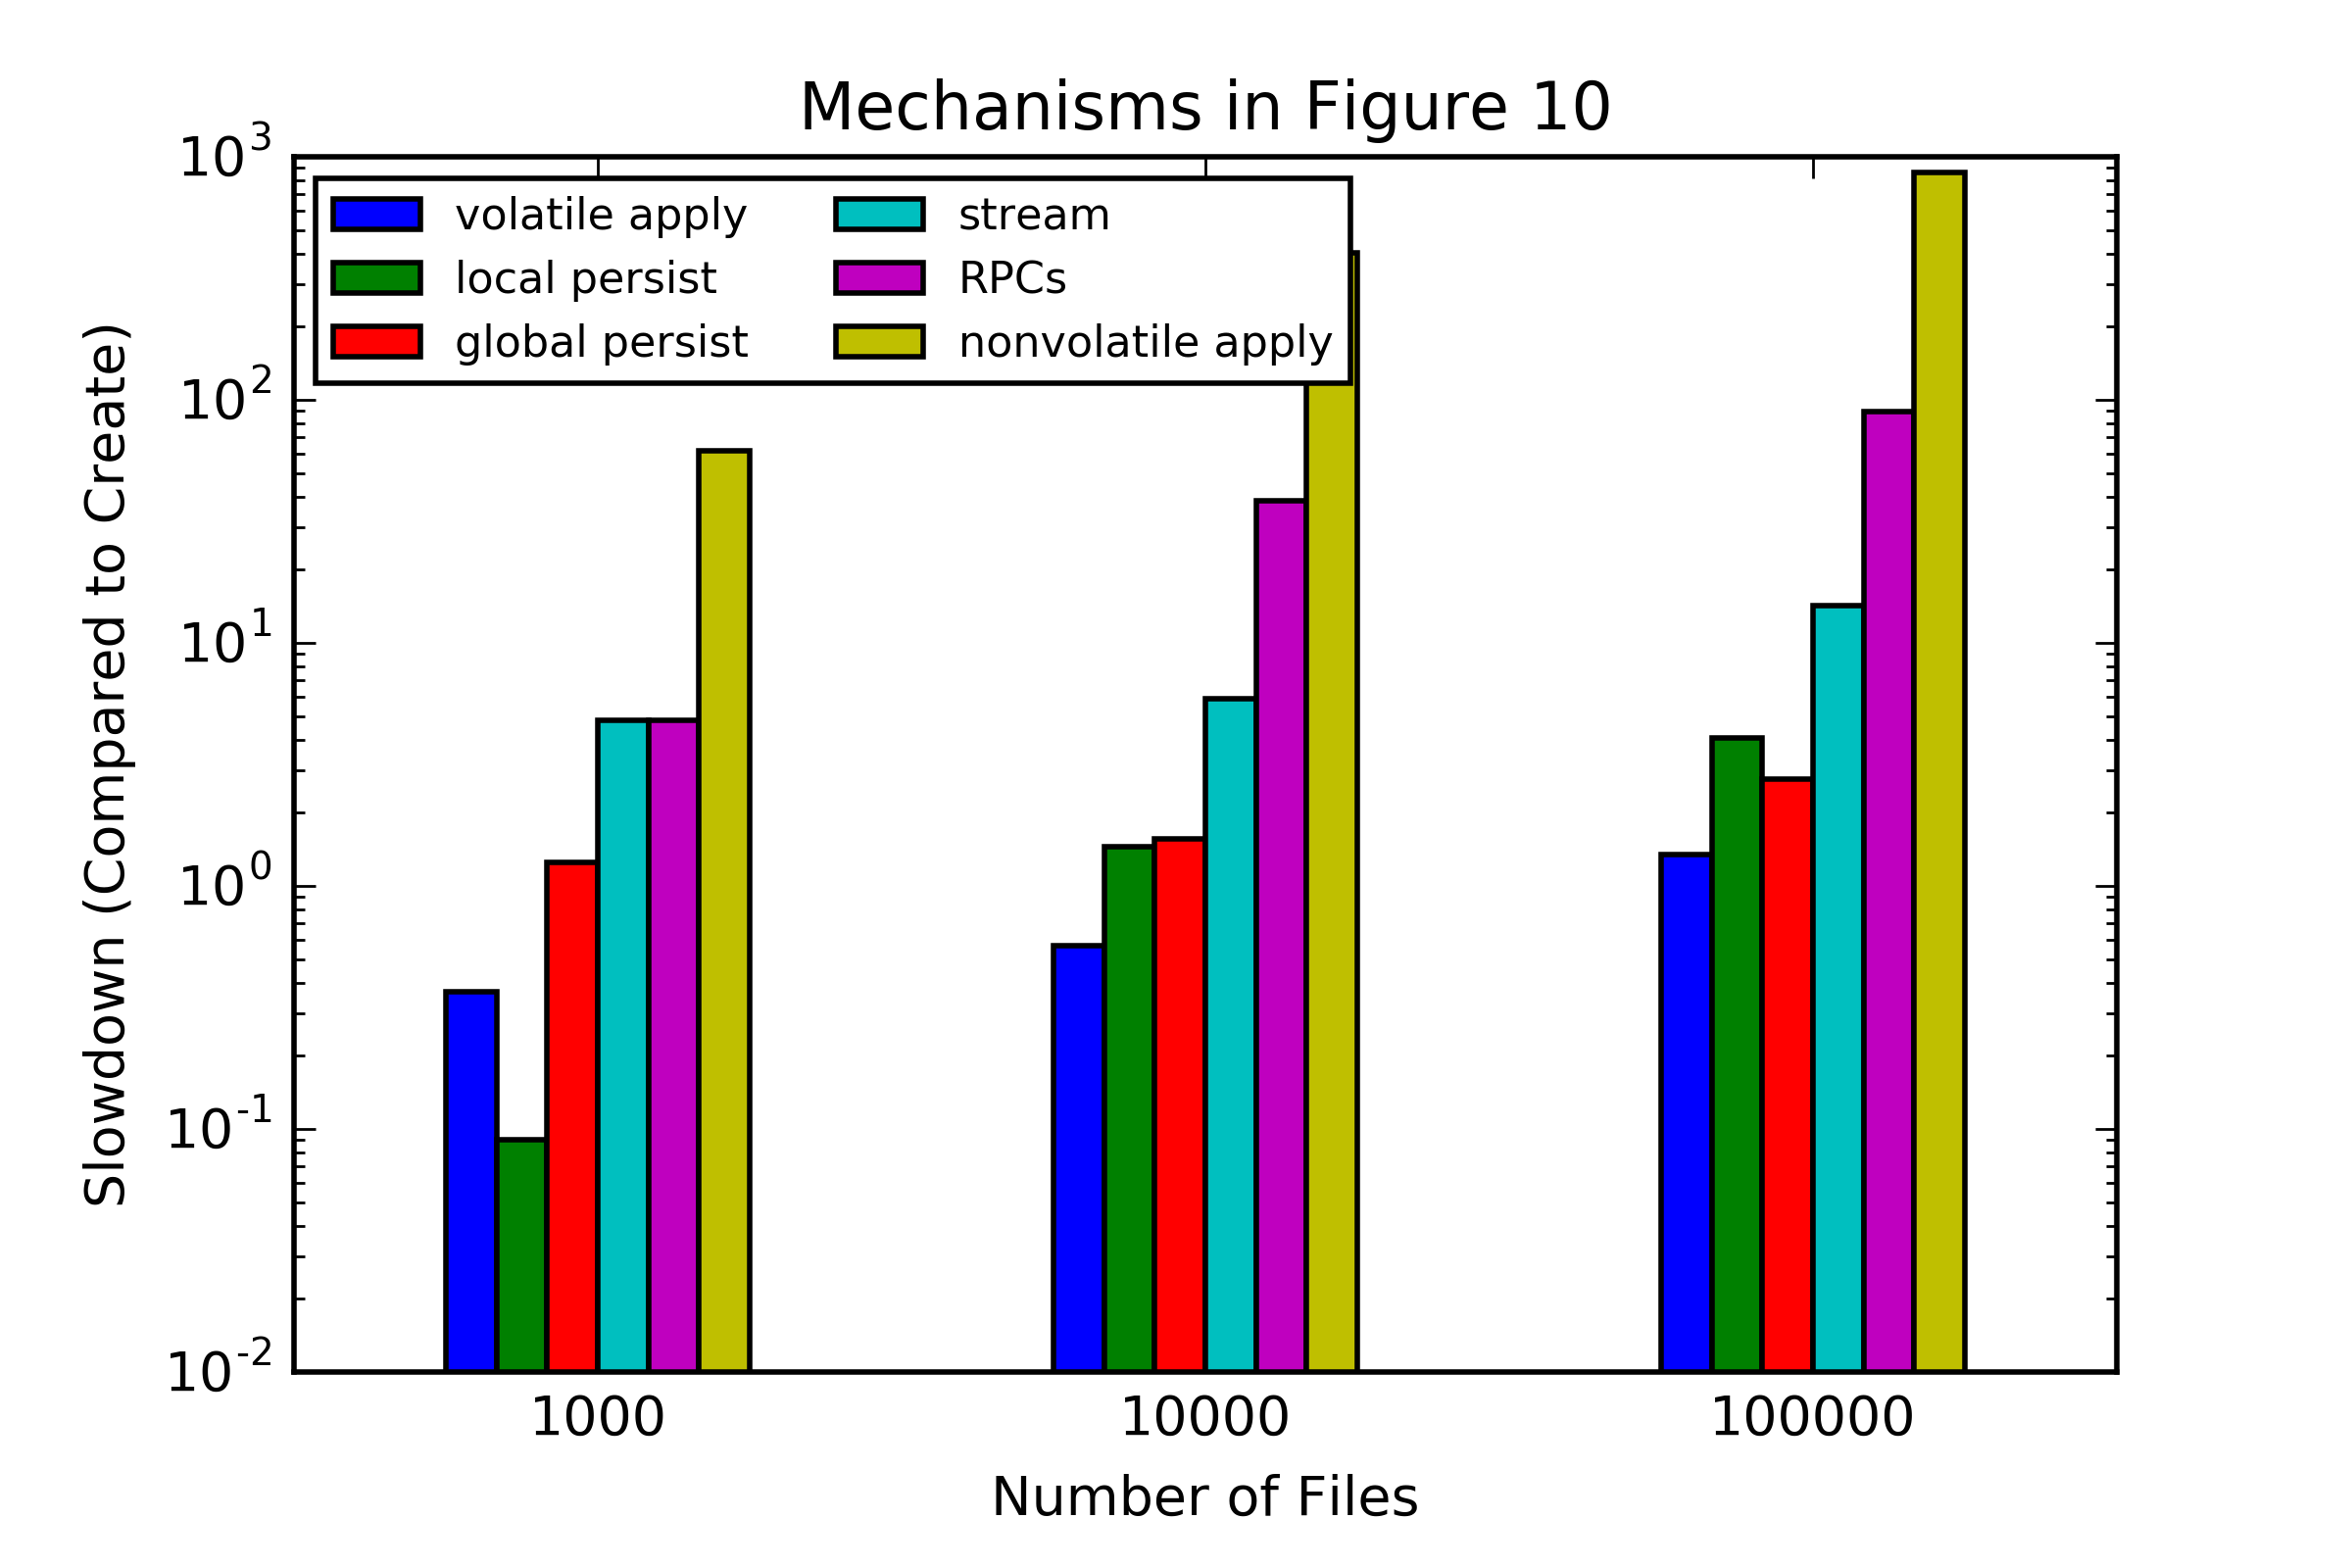
\includegraphics[width=1.0\linewidth]{graphs/slowdown-mechanisms.png}
\caption{}
\end{figure}
\begin{figure}[tb]
\centering
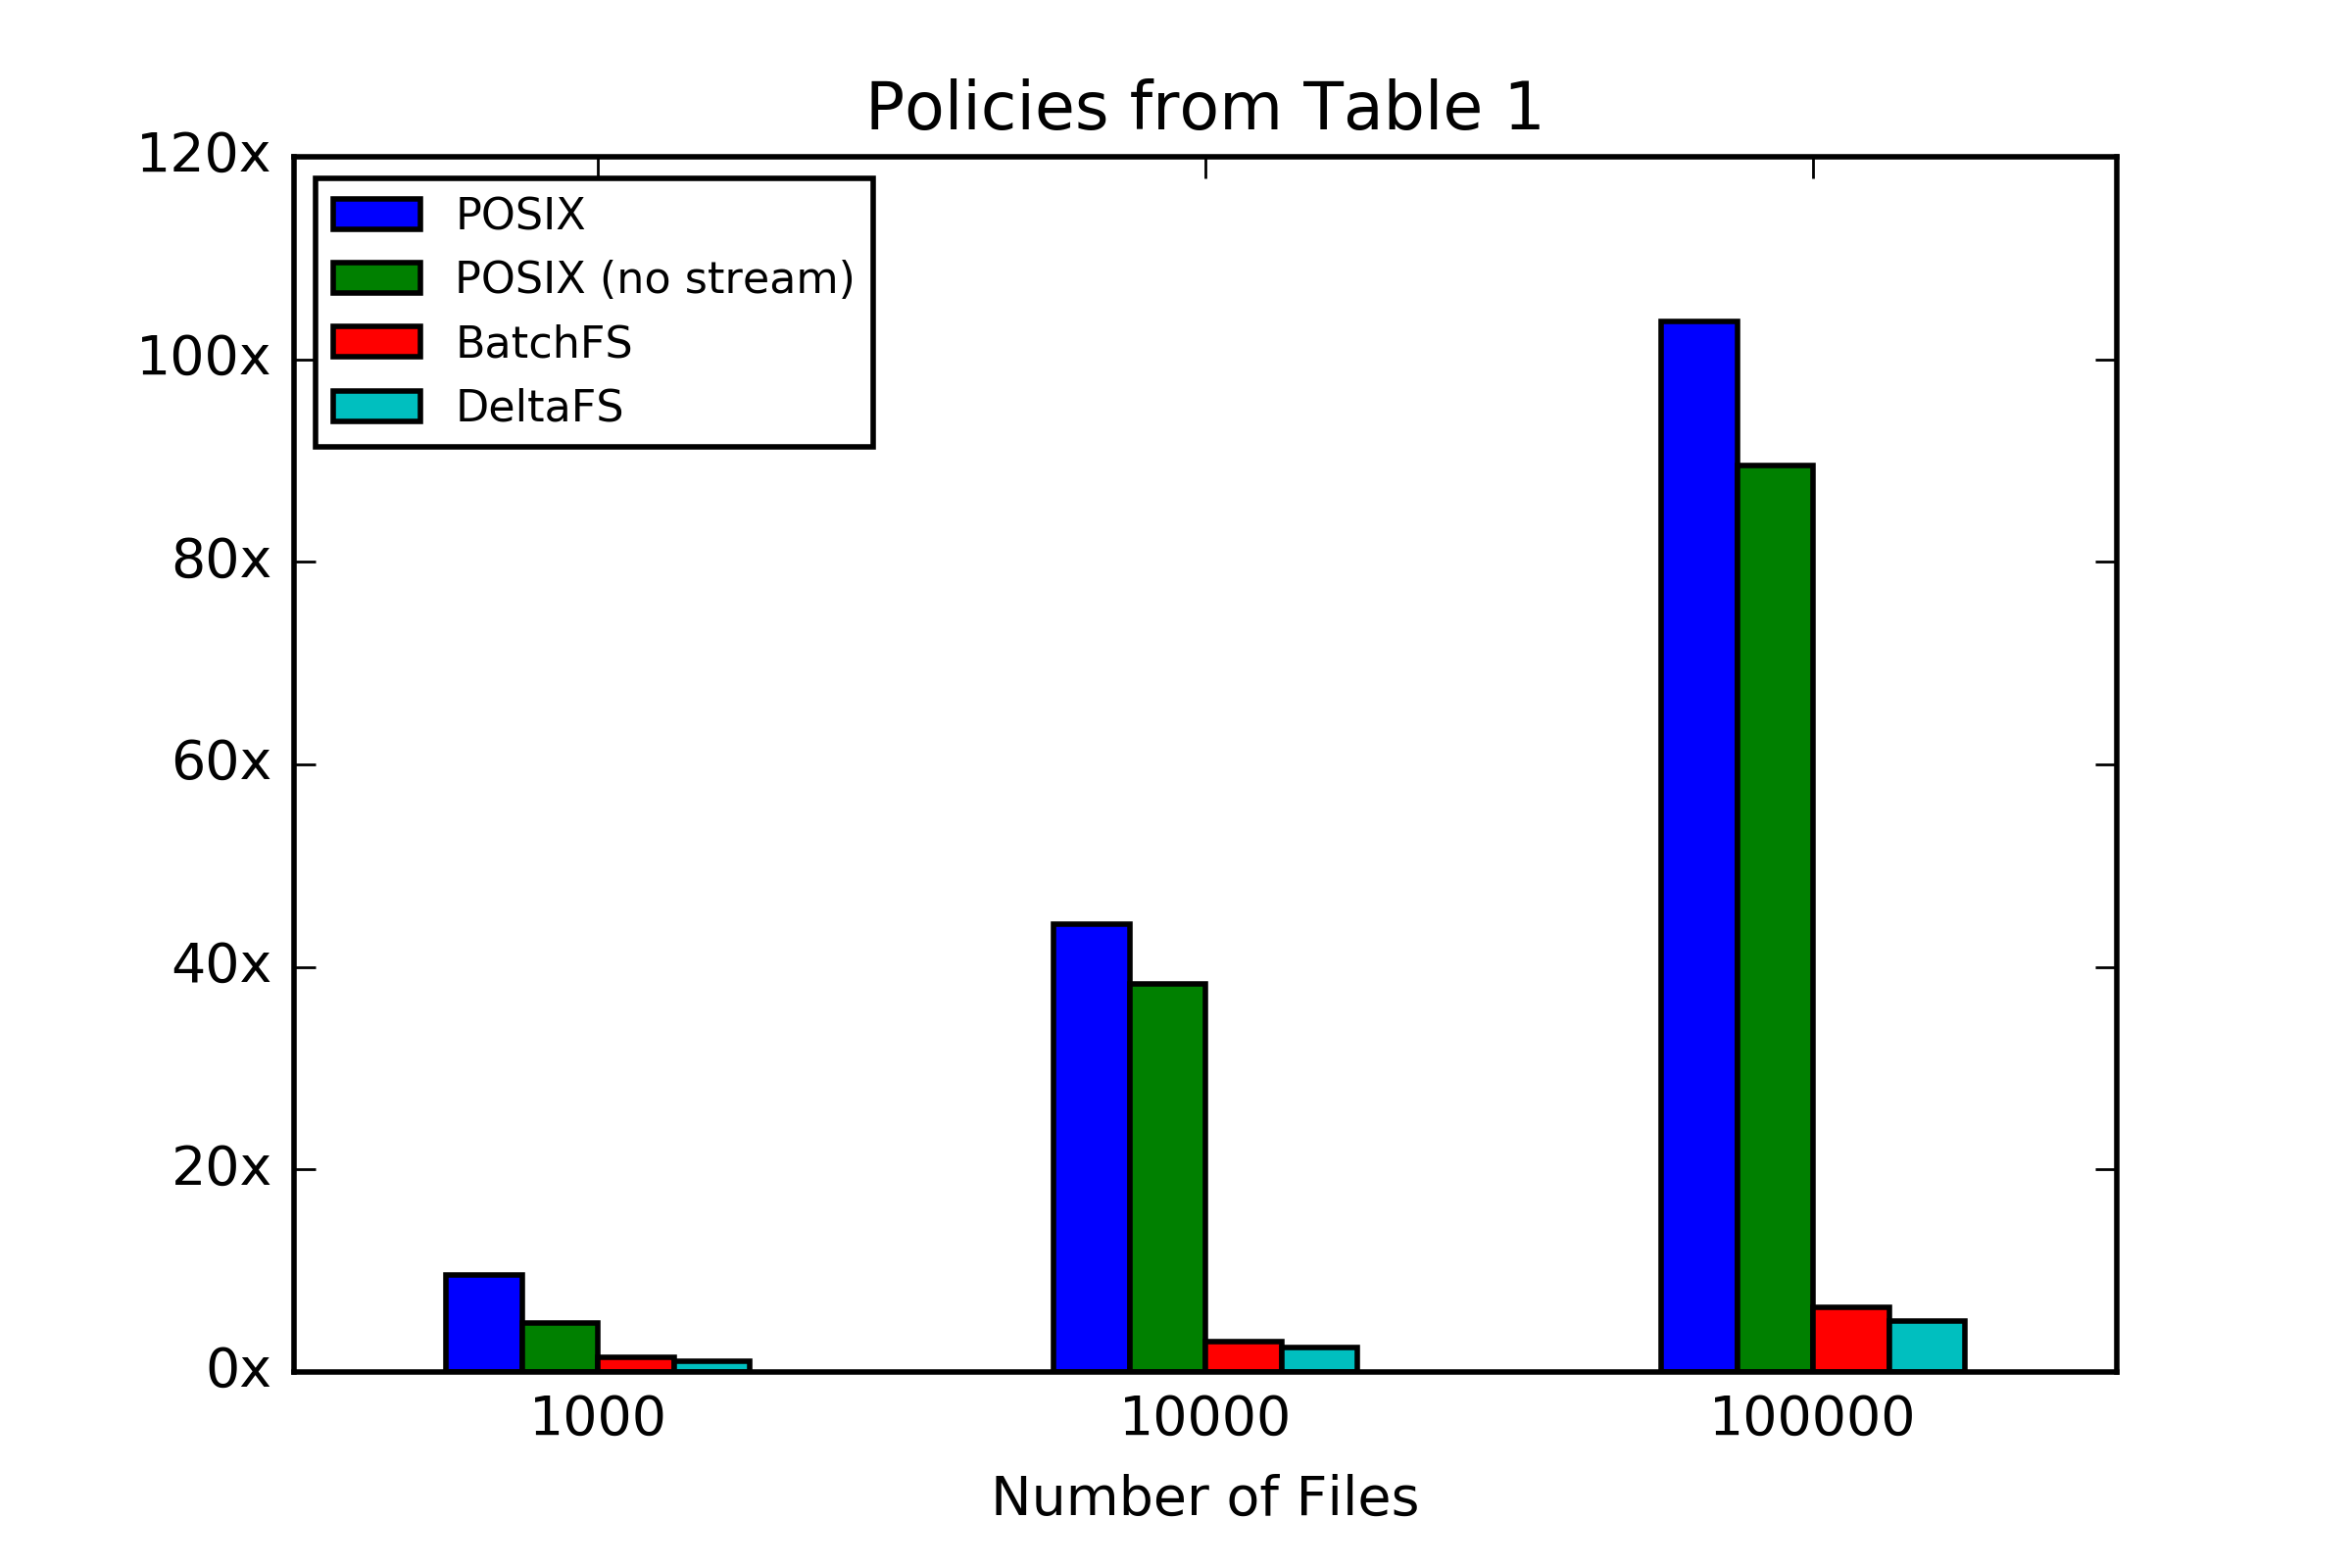
\includegraphics[width=1.0\linewidth]{graphs/slowdown-related-work.png}
\caption{}
\end{figure}
\begin{figure}[tb]
\centering
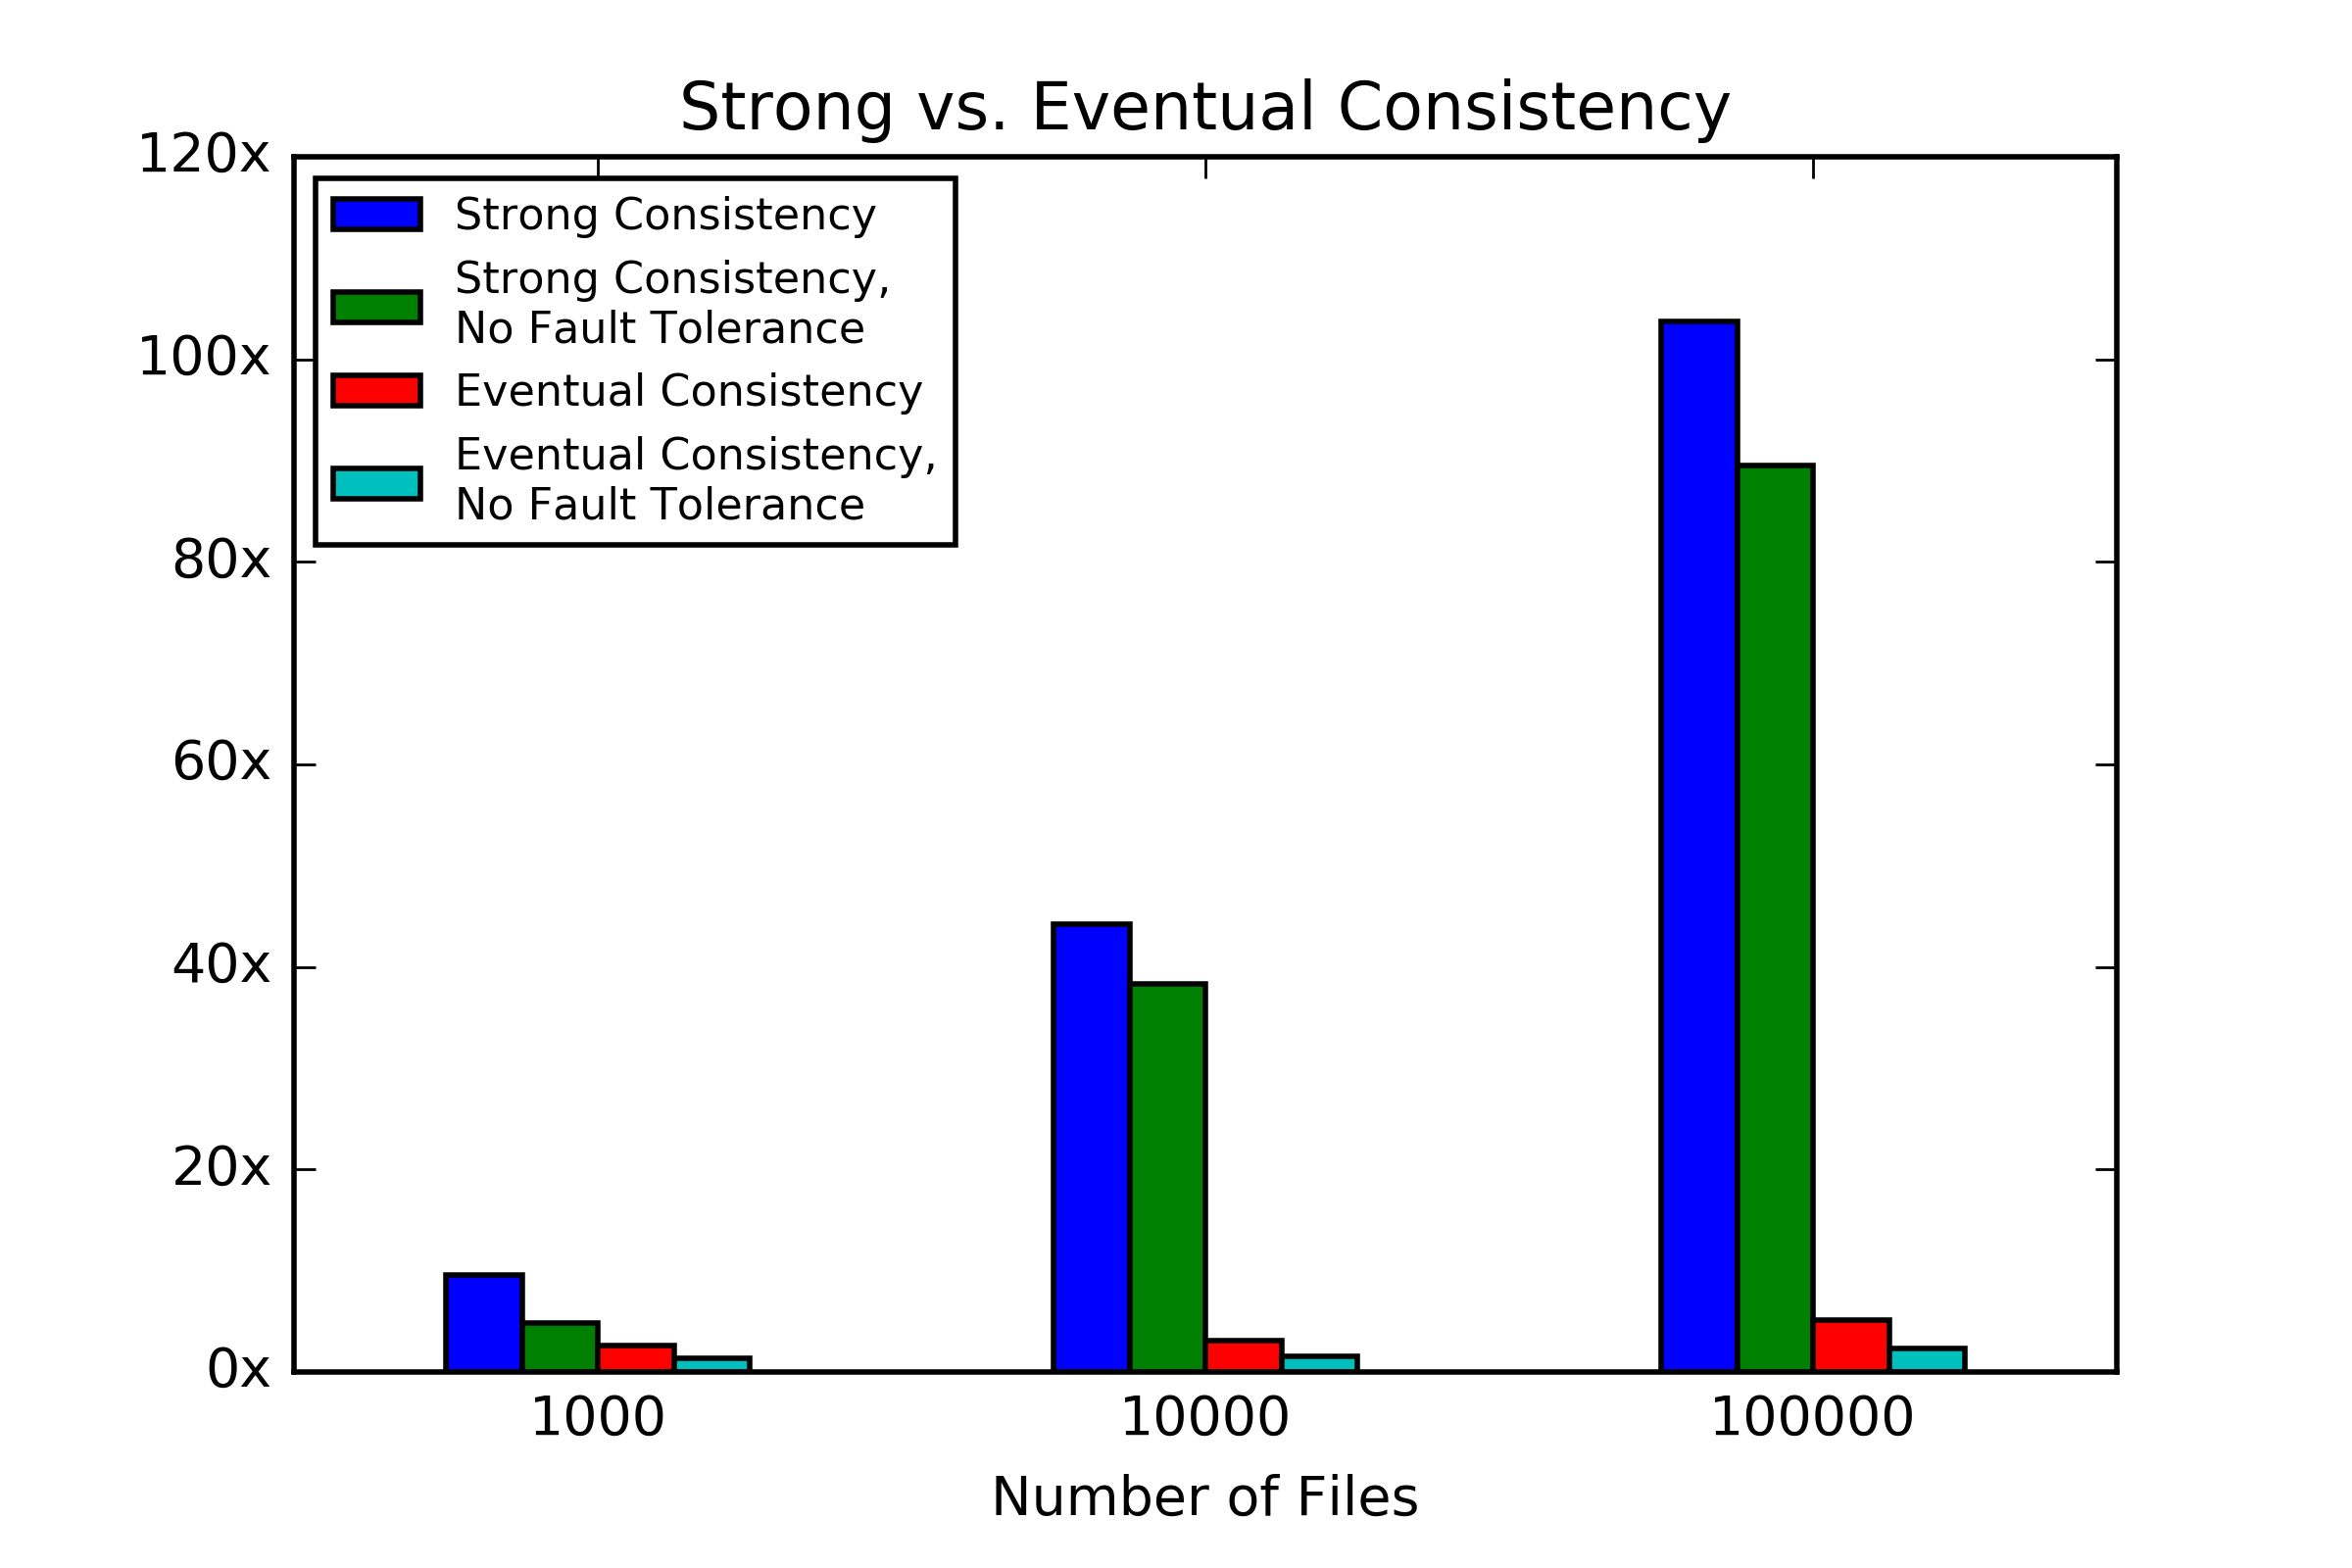
\includegraphics[width=1.0\linewidth]{graphs/slowdown-strong-v-eventual.png}
\caption{}
\end{figure}

\subsubsection{Per phase latencies}

%\section{notes}
%Linking clients into our custom libcephfs
%
%Use namespace's recursive data structure to put policies on subtrees
%- consistency: eventual vs. strong, global vs. local
%  - e.g., BatchFS/DeltaFS: eventual, local
%  - e.g., POSIX: strong, global
%  - e.g., PLFS: no consistency
%- fault tolerance: global vs. local
%  - e.g., CephFS: global
%  - e.g., BatchFS/DeltaFS: local
%
%Experimental Setup
%- Ceph: 9 OSDs, 1 MDS, 2 kernel client
%- Workload limitations: blah
%
%Workload: creates
%
%Baseline: 200K creates in the same directory
%- throughput: degrades at 950s
%- CPU utilization: more at 950s
%- inode cache: eviction dominate
%- inodes +- to cache: eviction dominate
%- per-disk throughput: RADOS not bottleneck
%
%Experiment 1: Interference
%
%\subsection{Baseline}
%Experiment 0: creates in the same directory
%- setup: why we use caching, we use the kernel client, how we circumvent max fragment size
%
%Experiment 0: creates with a stat
%- Hypothesis: metadata read pauses creates and requires a snapshot in time
%  - what is more of an overhead: pausing creates and getting a consistent view OR sucking up resources as it reads from RADOS?
%- can we delay snapshot?
%
%Experiment 1: creates with a readdir
%- Hypothesis: shows the cost of synchronization because on a write, the first client drops his caps
%- client0: create 100k, client1: stat at 2 mins
%
%Experiment 2: scale the number of files
%- See if the open/close spike occurs 
%- Try to see why open/close spike is allowed to happen
%- Try to disable all caching -- metadata writes don't ever re-use the inode -- we never ask for it again!
%- client0: create 100k, client1: touch at 2 mins
%
%Experiment 3: see how fast the cache satisfies a read
%- client0: create 100k, stat inodes
%- client0: create 100k, client1: stat inodes
%
%lient 0: creates, client 1 create(s)

\subsection{Isolation from EBUSY}
\subsection{Isolation from Global Writes, Cost of Overwrites}
\subsection{Partial Directory Listings}

\subsection{Macrobenchmarks}
updatedb: http://lists.ceph.com/pipermail/ceph-users-ceph.com/2015-July/002768.html


